%% LyX 2.3.6.1 created this file.  For more info, see http://www.lyx.org/.
%% Do not edit unless you really know what you are doing.
\documentclass[english]{article}
\usepackage[T1]{fontenc}
\usepackage[latin9]{inputenc}
\usepackage{geometry}
\geometry{verbose,tmargin=2.5cm,bmargin=2.5cm,lmargin=2.5cm,rmargin=2.5cm}
\usepackage{calc}
\usepackage{graphicx}

\makeatletter

%%%%%%%%%%%%%%%%%%%%%%%%%%%%%% LyX specific LaTeX commands.
%% Because html converters don't know tabularnewline
\providecommand{\tabularnewline}{\\}

\makeatother

\usepackage{babel}
\begin{document}
{[}SPLIT\_HERE{]}
\begin{enumerate}
\item \textbf{{[}HCI/PRELIM/9597/2017/P1/Q1{]} }

A web log,\texttt{ WEBLOG.txt}, keeps track of the date and time the
server is being accessed, and the client that accessed it. The client
is identified by either the host name or internet address. The format
of \texttt{WEBLOG.txt} is as follows: 
\noindent \begin{center}
\texttt{<host name>|<DD/MMM/YYYY:HH:MM:SS> }
\par\end{center}

or
\noindent \begin{center}
\texttt{<internet address>|<DD/MMM/YYYY:HH:MM:SS> }
\par\end{center}

Below is a sample of \texttt{WEBLOG.txt}: 

\noindent\fbox{\begin{minipage}[t]{1\columnwidth - 2\fboxsep - 2\fboxrule}%
\texttt{199.72.81.55|01/Jul/1995:00:00:01 }

\texttt{unicomp6.unicomp.net|01/Jul/1995:00:00:06 }

\texttt{199.120.110.21|01/Jul/1995:00:00:09 }

\texttt{burger.letters.com|01/Jul/1995:00:00:11} %
\end{minipage}}

The client address (host name or internet address) can appear multiple
times, depending on how many times it accessed the server. Similarly,
the date it accessed the server can be duplicated too because it can
access the server many times in a day. 

A summary report, SUMMARY.txt, is to be generated to list the \textbf{unique}
clients (hosts name/internet address) and the corresponding list of
\textbf{unique} dates that it has accessed the server, from the web
log, \texttt{WEBLOG.txt}. 

Below is a sample of \texttt{SUMMARY.txt}: 

\noindent\fbox{\begin{minipage}[t]{1\columnwidth - 2\fboxsep - 2\fboxrule}%
\texttt{199.72.81.55 01/Jul/1995,03/Jul/1995,04/Jul/1995 }

\texttt{Buger.letters.com 01/Jul/1995,05/Jul/1995}

\texttt{Computing.com 01/Jul/1995,02/Jul/1995,03/Jul/1995}%
\end{minipage}}

\subsection*{Task 1.1}

Write a procedure \texttt{ReadLog()} to read \texttt{WEBLOG.txt},
using a suitable data structure(s), and prepare the log information
to create \texttt{SUMMARY.txt}.

\subsection*{Evidence 1 }

Your \texttt{ReadLog()} procedure code. \hfill{}{[}4{]}

\subsection*{Task 1.2 }

Write a procedure \texttt{ProcessLog()} to generate \texttt{SUMMARY.txt}. 

\subsection*{Evidence 2}

Your \texttt{ProcessLog()} procedure code.\hfill{} {[}4{]}

\subsection*{Evidence 3 }

Screenshot of \texttt{SUMMARY.txt} after running the program. \hfill{}{[}1{]}

\subsection*{Task 1.3 }

Add code to your Task 1.2 program to output to screen the highest
number of days the server was accessed by any client, and the corresponding
client(s). Below is a sample of screen output:

\noindent\begin{minipage}[t]{1\columnwidth}%
\texttt{Highest frequency (days): 3 }

\texttt{Accessed by: }

\texttt{199.72.81.55}

\texttt{Computing.com}%
\end{minipage}

\subsection*{Evidence 4}

Your program code for Task 1.3.\hfill{} {[}4{]}

\subsection*{Evidence 5}

Screenshot of the program output. \hfill{}{[}1{]}

{[}SPLIT\_HERE{]}
\item \textbf{{[}HCI/PRELIM/9597/2017/P1/Q2{]} }

The files \texttt{CUPS-SOLD1.txt} and \texttt{CUPS-SOLD2.txt} contain
the daily total number of cups of coffee sold at a caf� over a period
of 50 days. The task is to read the daily sales from the file and
to allow a search for a specific sales figure. You will program two
different search algorithms: 
\begin{itemize}
\item Linear Search 
\item Binary Search 
\end{itemize}

\subsection*{Task 2.1 }

Write program code that repeatedly: 
\begin{itemize}
\item displays a menu with the following options:
\noindent \begin{center}
\begin{tabular}{|l|}
\hline 
1. Read File\tabularnewline
2. Linear Search\tabularnewline
3. Binary Search\tabularnewline
4. End\tabularnewline
\hline 
\end{tabular}
\par\end{center}
\item calls an appropriate procedure/function depending on the user\textquoteright s
option.
\end{itemize}

\subsection*{Evidence 6 }

Program code for Task 2.1. \hfill{}{[}3{]}

\subsection*{Task 2.2 }

Write the program code for a procedure to implement menu option 1. 

\subsection*{Evidence 7 }

Program code for menu option 1. \hfill{}{[}2{]}

Options 2 and 3 will perform a search for a specified sales figure
and display a message to indicate if it is found or not. 

\subsection*{Task 2.3}

Write program code as a function to implement the linear search for
menu option 2. The function will return 0 if the sales figure is found,
or -1 if it is not found. 

The program will: 
\begin{itemize}
\item Input a sales figure 
\item Use the function \texttt{LinearSearch} 
\item Report whether or not this sales figure was found.
\end{itemize}
Use \texttt{CUPS-SOLD1.txt} to test your program code. 

Run the program two times. Use the following inputs: \texttt{167}
and \texttt{405}. 

\subsection*{Evidence 8}
\begin{itemize}
\item Program code for menu option 2.
\item Screenshots showing the output from menu option 2. \hfill{}{[}5{]}
\end{itemize}

\subsection*{Task 2.4 }

Write program code as a function to implement the binary search for
menu option 3. The function will return \texttt{0} if the sales figure
is found, or \texttt{-1} if it is not found. 

\textbf{{*}Hint: Do not use any pre-defined sort function e.g. sort()
in your program code.}

The program will: 
\begin{itemize}
\item Input a sales figure
\item Use the function \texttt{BinarySearch} 
\item Report whether or not this sales figure was found.
\end{itemize}
Use \texttt{CUPS-SOLD1.txt} to test your program code. Run the program
two times. Use the following inputs: \texttt{366} and \texttt{123}. 

\subsection*{Evidence 9 }
\begin{itemize}
\item Program code for menu option 3. 
\item Screenshots showing the output from menu option 3. \hfill{}{[}10{]}
\end{itemize}

\subsection*{Task 2.5}

Amend your program code for the linear search function so that if
the specified sales figure exists, the number of day(s) with this
sales figure is also reported. 

Use the file \texttt{CUPS-SOLD2.txt} to test your program. 

\subsection*{Evidence 10 }

The amended program code for menu option 2. \hfill{}{[}3{]}

\subsection*{Task 2.6}

Study the contents of \texttt{CUPS-SOLD2.txt} and then devise a set
of three test cases with the sales figures to be used for testing
the amended code. Evidence 11 A screenshot for each test case you
considered. Annotate the screenshot explaining the purpose of each
test. \hfill{}{[}3{]}

{[}SPLIT\_HERE{]}
\item \textbf{{[}HCI/PRELIM/9597/2017/P1/Q3{]} }

An application is to be created to store a Football League table data.
The team names are stored in the file \texttt{TEAMS.txt}. The results
of the football matches are provided in file \texttt{RESULTS.txt}.

Each match data takes up one line, for example: \texttt{MadUnited
2 Chelsand 1 }

That is, \texttt{MadUnited} won \texttt{Chelsand}, scoring two goals
and conceding one goal, or Chelsand lost to Mad United, scoring one
goal and conceding two goals. 

The League table that needs to be created has the following information: 
\noindent \begin{center}
\begin{tabular}{llllllllll}
\textbf{Team} &  & \textbf{P} & \textbf{W} & \textbf{D} & \textbf{L} & \textbf{GF} & \textbf{GA} & \textbf{GD} & \textbf{Points}\tabularnewline
\hline 
\texttt{MadUnited} &  & \texttt{4} & \texttt{3} & \texttt{1} & \texttt{0} & \texttt{8} & \texttt{3} & \texttt{5} & \texttt{10}\tabularnewline
\texttt{Chelsand} &  & \texttt{4} & \texttt{2} & \texttt{1} & \texttt{1} & \texttt{10} & \texttt{7} & \texttt{3} & \texttt{7}\tabularnewline
\texttt{Lovepool} &  & \texttt{5} & \texttt{2} & \texttt{1} & \texttt{2} & \texttt{4} & \texttt{6} & \texttt{-2} & \texttt{7}\tabularnewline
$\dots$ &  &  &  &  &  &  &  &  & \tabularnewline
$\dots$ &  &  &  &  &  &  &  &  & \tabularnewline
\end{tabular}
\par\end{center}

\noindent %
\noindent\begin{minipage}[t]{1\columnwidth}%
\textbf{Legend}: 

\textbf{P} -- games played 

\textbf{W} -- games won

\textbf{D} -- games drawn

\textbf{L} -- games lost 

\textbf{GF} -- goals for (scored against opponents)

\textbf{GA} -- goals against (goals conceded by team)

\textbf{GD} -- goal difference, i.e. GD = GF -- GA

\textbf{Points} -- computed based on 3 points per win, 1 point per
draw and zero points per loss%
\end{minipage}

\subsection*{Task 3.1 }

Write program code for a procedure \texttt{CreateUpdateFile} which
does the following: 
\begin{itemize}
\item the program reads the \textbf{first} match results from \texttt{RESULTS.txt}
\item appends to the results of each team to a text file \texttt{NEWFILE.txt}
with the following information: team name, result of match (W/D/L),
goals for (GF), goals against (GA)
\item for e.g. the data \textquotedblleft \texttt{MadUnited 2 Chelsand 1}\textquotedblright{}
will result in the following two records to be appended to \texttt{NEWFILE.txt}.

\noindent\begin{minipage}[t]{1\columnwidth}%
\texttt{MadUnited,W,2,1}

\texttt{Chelsand,L,1,2}%
\end{minipage}
\end{itemize}

\subsection*{Evidence 12 }

Your CreateUpdateFile program code. \hfill{}{[}5{]}

\subsection*{Task 3.2 }

Amend your \texttt{CreateUpdateFile} program code from Task 3.1 so
that all the match results are read from \texttt{RESULTS.txt}, and
the \texttt{NEWFILE.txt} updated accordingly. 

\subsection*{Evidence 13 }

Your program code for the amended procedure \texttt{CreateUpdateFile}.
\hfill{}{[}2{]}

\subsection*{Evidence 14 }

2 screenshots of \texttt{NEWFILE.txt} showing first 10 and last 10
records. \hfill{} {[}2{]}

\subsection*{Task 3.3 }

Write program code for a function \texttt{ComputeTeamStat} which does
the following: 
\begin{itemize}
\item receives a team name as a parameter 
\item the function searches the file \texttt{NEWFILE.txt} for all occurrences
of that team
\item calculates and outputs the team\textquoteright s league table information, 

e.g. for team \textquoteleft \texttt{MadUnited}\textquoteright , it
may output the following: 
\noindent \begin{center}
\begin{tabular}{llllllllll}
\textbf{Team} &  & \textbf{P} & \textbf{W} & \textbf{D} & \textbf{L} & \textbf{GF} & \textbf{GA} & \textbf{GD} & \textbf{Points}\tabularnewline
\hline 
\texttt{MadUnited} &  & \texttt{4} & \texttt{3} & \texttt{1} & \texttt{0} & \texttt{8} & \texttt{3} & \texttt{5} & \texttt{10}\tabularnewline
\end{tabular}
\par\end{center}
\end{itemize}

\subsection*{Evidence 15 }

Your \texttt{ComputeTeamStat} program code.\hfill{} {[}6{]}

\subsection*{Evidence 16 }

A screenshot showing the output for the team \texttt{Everlong}. \hfill{}{[}1{]}

\subsection*{Task 3.4 }

Write program code for a procedure \texttt{GenerateTable} which does
the following: 
\begin{itemize}
\item reads the data from files \texttt{TEAMS.txt} and \texttt{NEWFILE.txt}
\item and makes use of the function \texttt{ComputeTeamStat} from Task 3.3 
\item to output the complete league table information ordered by the team
with the highest points first. If two or more teams having the same
points, team having more goal difference (GD) will be listed first. 
\end{itemize}

\subsection*{Evidence 17 }

Your \texttt{GenerateTable} program code.\hfill{} {[}7{]}

\subsection*{Evidence 18 }

A screenshot showing the output for the complete League table.\hfill{}
{[}2{]}

{[}SPLIT\_HERE{]}
\item \textbf{{[}HCI/PRELIM/9597/2017/P1/Q4{]} }

The task is to store a dataset of students\textquoteright{} names
and test scores (max size of 20 students) as a binary tree structure.
The text file \texttt{SCORES.txt} stores the students\textquoteright{}
names and test scores in the following format: 
\noindent \begin{center}
\texttt{<Student Name>|<Score> }
\par\end{center}

All test scores are integer values in the range 0 to 100 inclusive. 

The program will use a user-defined type \texttt{Node} for each node
defined as follows: 
\noindent \begin{center}
\begin{tabular}{|c|c|c|}
\hline 
\textbf{Identifier} & \textbf{Data Type} & \textbf{Description}\tabularnewline
\hline 
\texttt{LeftP} & \texttt{INTEGER} & The left pointer for the node\tabularnewline
\hline 
\texttt{Name} & \texttt{STRING} & The name of the student\tabularnewline
\hline 
\texttt{Score} & \texttt{INTEGER} & The score of the student\tabularnewline
\hline 
\texttt{RightP} & \texttt{INTEGER} & The right pointer for the node\tabularnewline
\hline 
\end{tabular}
\par\end{center}

A linked list is maintained of all the unused nodes which do not form
part of the tree. The first available node which is used for a new
student is indicated by \texttt{NextFreePosition}. Nodes in the unused
list are linked using their left pointers.

The binary tree and linked list are implemented using variables as
follows:
\noindent \begin{center}
\begin{tabular}{|c|c|c|}
\hline 
\textbf{Identifier} & \textbf{Data Type} & \textbf{Description}\tabularnewline
\hline 
ThisTree & ARRAY{[}20{]}: Node & The tree data\tabularnewline
\hline 
Root & INTEGER & Index for the root position of the array\tabularnewline
\hline 
NextFreePosition & INTEGER & Index for the next unused node\tabularnewline
\hline 
\end{tabular}
\par\end{center}

\begin{center}
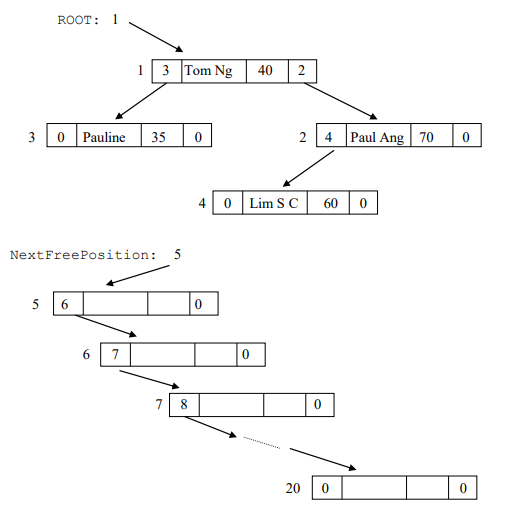
\includegraphics[width=0.5\paperwidth]{C:/Users/Admin/Desktop/Github/question_bank/LyX/static/img/9597-HCI-2017-P1-Q4-1}
\par\end{center}

The diagram shows the binary tree with the students\textquoteright{}
scores 40, 70, 35 and 60 (added in that order) and linked list of
unused nodes after the four students\textquoteright{} scores have
been added. 

\subsection*{Task 4.1 }

Write the program code to declare all the required variables and create
the initial linked list which contains all 20 nodes. Add statement(s)
to initialize the empty tree. 

\subsection*{Evidence 19 }

Your program code for Task 4.1. \hfill{}{[}8{]}

\subsection*{Task 4.2}

Write a non-recursive procedure \texttt{AddNodeToTree} to add a new
node with student\textquoteright s name and score into the binary
tree structure. 

\subsection*{Evidence 20}

Your program code for Task 4.2.\hfill{} {[}8{]}

\subsection*{Task 4.3 }

Write a procedure \texttt{OutputData} which displays the value of
\texttt{Root}, the value of \texttt{NextFreePosition} and the contents
of \texttt{ThisTree} in index order.

\subsection*{Evidence 21 }

Your program code for Task 4.3.\hfill{} {[}5{]}

\subsection*{Task 4.4 }

Write a main program to: 
\begin{itemize}
\item construct a binary search tree using the data provided in the text
file SCORES.txt by calling procedure \texttt{AddNodeToTree}. 
\item Your program will then call procedure \texttt{OutputData}. 
\end{itemize}

\subsection*{Evidence 22 }

Your program code for Task 4.4.\hfill{} {[}4{]}

\subsection*{Evidence 23 }

Screenshot showing the output from running the program in Task 4.4.\hfill{}
{[}4{]}

\subsection*{Task 4.5}

Write a recursive procedure \texttt{RankList} to output students\textquoteright{}
names and scores in descending scores order. Include a call to the
procedure from your main program. Evidence 24 Your program code for
Task 4.5.\hfill{} {[}4{]}

\subsection*{Evidence 25 }

Provide a screenshot showing students\textquoteright{} names and scores
in descending scores order. \hfill{}{[}2{]}

{[}SPLIT\_HERE{]}
\end{enumerate}

\end{document}
